\documentclass[a4paper, 12pt, twoside]{book}
	\PassOptionsToPackage{table}{xcolor}
	\usepackage[export]{adjustbox}
	\usepackage[english,ngerman]{babel}
	\usepackage{amsmath, url}
	\usepackage[utf8]{inputenc}
	\usepackage[T1]{fontenc}
	\usepackage{import}
	\usepackage{graphicx}
	\usepackage{subcaption}
	\usepackage{verbatim}
	\usepackage{float}
	\usepackage[headheight=12pt]{geometry}
	\usepackage{fancyhdr}
	\usepackage{subfiles}
	\usepackage{float}
	\usepackage[table,xcdraw,dvipsnames]{xcolor}
  \usepackage{amsmath}
	\usepackage{wrapfig}
\usepackage[rightcaption]{sidecap}
\usepackage[font=small,labelfont=bf,tableposition=top]{caption}
	%  Bibliographie
	\usepackage{bibgerm} % Umlaute in BibTeX
%\usepackage[style=authortitle-icomp]{biblatex}
\bibliographystyle{ieeetr} 
\usepackage[babel,german=guillemets]{csquotes}

	

	\pagestyle{fancy}
	\fancyhf{}
	\fancyhead[LE,RO]{Baran Avinc}
	\fancyhead[RE,LO]{Masterarbeit}
	\fancyfoot[LE,RO]{\vspace{0.05cm}\thepage}
	%\fancyfoot[RE,LO]{\vspace{0.05cm}\includegraphics[width=0.1\textwidth]{Bilder/TU-Berlin-Logo.pdf}}
	\renewcommand{\headrulewidth}{1pt}
	\renewcommand{\headrule}{\hbox to\headwidth{\color{RoyalPurple}\leaders\hrule height 				\headrulewidth\hfill}}
	\renewcommand{\footrulewidth}{1pt}
	\renewcommand{\footrule}{\hbox to\headwidth{\color{RoyalPurple}\leaders\hrule height \footrulewidth\hfill}}
	\pagestyle{fancy}


	


  	%\includegraphics[width=0.1\textwidth]{Bilder/TU-Berlin-Logo.pdf}

	





\begin{document}
	
\begin{titlepage}
		\pagestyle{fancy}
		\raggedleft{\includegraphics[width=0.2\textwidth]{Bilder/TU-Berlin-Logo.pdf}} \\
		\vspace{1cm} 
		\centering Fakultät II - Mathematik und Naturwissenschaften \\
		\centering Institut für Festkörperphysik \\
		\centering AG Kneissl \\
		\vspace{0.5cm}
		\centering\textbf{\large Masterarbeit zum Thema}\\
		\vspace{1cm} 
		\noindent{\color{RoyalPurple}\rule{\textwidth}{1pt}} \\
		\vspace{0.5cm} 
		\centering\textbf{\large Untersuchung der optischen Polarisation und internen Quanteneffizienz von AlGaN Quantenfilmen mittels temperatur- und leistungsabhängiger Photolumineszenzspektroskopie} \\
		\vspace{0.25cm} 
		\noindent{\color{RoyalPurple}\rule{\textwidth}{1pt}} \\
		\vspace{1cm}
		\centering \emph{ \large{Masterarbeit}} \\
		\centering Baran Avinc \\
		\vspace{1cm}
		\centering \emph{ \large{Gutachter}} \\
		\centering Prof. Dr. Michael Kneissl \\
		\centering Prof. Dr. Axel Hoffmann  \\
		\vspace{0.5cm} 
		\centering \emph{ \large{Betreuer}} \\
		\centering Christoph Reich \\
		\centering Bettina Belde \\
		\vspace{1cm}
		\centering  \today \\
\end{titlepage}



	\tableofcontents\thispagestyle{fancy}
	
\chapter{Einleitung}
\thispagestyle{fancy}

\begin{quote}
In the spirit of Alfred Nobel the Prize rewards an invention of greatest benefit to mankind; using blue LEDs, white Light can be created in a new way.\end{quote}
Dieser Satz, den die Schwedische Akademie der Künste nach der Vergabe des Nobelpreises an die Entwicklung der blauen LED(kurz, light emitting diode) im Jahr 2014 an die Presse veröffentlichte, fasst treffend zusammen, wie hoch die Bedeutung der auf Halbleiterkristallen basierenden optischen Bauelemente ist.
LEDs nehmen einen fundamentalen und immer bedeutender werdenden Teil unseres alltäglichen Lebens ein. Ausgezeichnet durch ihre hervorragende Effizienz, konkurrenzlosen Lebensdauer und geringen Dimension übernimmt sie durch eine immer höher werdenden Lichtausbeute zusehends neue Anwendungsbereiche. 
%Seit jeher etabliert in den Bereichen der optischen Datenübertragung und Leuchtanzeige schreiten immer mehr andere Wellenlängenbereiche in den Fokus der weltweiten Forschung. 
Insbesondere auf Gallium Nitrid (GaN) basierende Halbleitermaterialien haben einen bahnbrechenden Weg hingelegt, der zur Entwicklung von hoch effizienten und leuchtstarken blauen LEDs führte und ebenfalls Grundlage für die Entwicklung in andere hochenergetische Wellenlängenbereiche darstellt~\cite{risk}.
So ebnet GaN auch den Weg für die Erzeugung von ultraviolet emittierenden Leuchtdioden. Der ultraviolette Spektralbereich, der sich unterteilt in den UV-A (400 nm bis 320 nm), UV-B (320 nm bis 280) und UV-C Bereich (280 nm bis 200 nm) ist bedeutend für eine sehr hohe Anzahl spezieller Anwendungsbereiche. Beispielsweise bieten sich UV-Leds an die bisher für Wasseraufbereitung genutzten Quecksilberdampflampen zu ersetzen, für deren Betrieb Hochspannungsnetzteile verwendet werden, die einen mobilen Einsatz erheblich erschweren können. Hier könnten UV-LEDs Abhilfe verschaffen, die durch ihr kleines Format und durch die niedrigen Betriebsspannungen einen Mobileneinsatz ermöglichen. Ein weiteres Anwendungsgebiet ist die industrielle Aushärtung/Aufbrechung von Lacken und die Gasdetektion. 
\newline
UV-LEDs leiden aber an einer geringen Effizienz die quantitativ als Externe Quanteneffizienz beschrieben wird. Die Gründe hierfür sind vielfältig. LEDs bestehen aus einer Viezahl an Schichten, die unterschiedlichen Funktionen dienen. Diese Schichten werden auf Substraten aufgewachsen. Daher ist eine hohe Substratqualität für die optischen Eigenschaften entscheidend. Eine geringe Defektdichte im Substrat geht einher mit einer ebenfalls geringen Defektdichte in den aufgewachsenen Schichten. Ein weiteres Problem im Zusammenhang mit den geringen Defektdichten, ist ein Mangel an geeigneten Substratmaterialien. So werden aufgrund des Preises und des Mangels an AlN Substrate auf Saphir Substrate ausgewichen. Durch die hohe Gitterfehlanpassung, ist AlN oder AlGaN nicht vollverspannt aufwachsbar. Bedeutet die Schichten relaxieren, was wiederum zur Entstehung von Defekten führt. 








	

\thispagestyle{fancy}

\section{Bandstruktur von Gruppe-III Nitriden}

Die wichtige Gruppe der III-Nitridhalbleiter setzt sich aus den Metallen
der dritten Hauptgruppe Aluminium (Al), Gallium (Ga) und Indium (In) zusammen.
Der Schwerpunkt dieser Arbeit liegt auf dem AlGaN-Materialsystem mit hohen Al-Konzentration. Das Mischverhältnis bestimmt hierbei die Bandlückenergie des Verbindungshalbleiters. Durch die unterschiedlichen Bandlückenergien von Aluminium mit 6.03 eV~\cite{fenaln} und GaN mit 3.4 eV~\cite{pipr} eignet sich AlGaN besonders für die Emission im Wellenlängenbereich von UV-A bis UV-C. 
Die Bandlückenenergie von AlGaN lässt sich durch Interpolation der binären Energien von GaN und AlN in Abhängigkeit des Kompositionsverhältnisses x berechnen, wobei ein zusätzlicher Bowing-Parameter für die nichtlineare Abweichung hinzugefügt wird. 

\begin{equation}
    E_{Al_{x}Ga{1-x}N} = E_{AlN} \cdot x + E_{GaN} \cdot (1-x) - b_{AlGaN} \cdot x \cdot (1-x) 
\end{equation}


\newpage
\section{Polarisationsfeld und QCSE in III/V Halbleitern}

Die Gruppe der III-Nitrid-Halbleiter kristallisiert in der Wurtzitstruktur. Anschaulich bedeutet dies, dass ausgehend von der hexagonal dichtesten Kugelpackung in Doppellagen, die Gruppe-III-Metallen und Stickstoff (N) sich entlang der c-Achse in der Abfolge A-B-A-B anordnen~\cite{buchc} wie in Abb. 2.1 dargestellt ist. 
\newline
Aufgrund der fehlenden Inversionssymmetrie und stark unterschiedlichen Elektronegativitäten des Stickstoffs und der entsprechenden Gruppe III-Metalle bilden sich Polarisationsfelder aus, die entlang der auf der Basalebende stehenden c-Achse verlaufen. Hier unterscheidet man zwischen zwei Arten von Polarisationsfeldern, die spontane Polarisation $ \vec{P}^{sp} $ und die piezoelektrische Polarisation $ \vec{P}^{pz} $.
\newline\newline
Die spontante Polarisation entsteht durch Dipolmomente im Kristall die sich aufgrund von ungleichen Bindungslängen nicht komplett aufheben. Ursprung der 
Dipolmomente im AlGaN sind die unterschiedlichen Elektronegativitäten zwischen den III-V Elementen und bedingt durch die angestrebte Minimierung der Gesamtenergie, kommt es zur Abweichung vom idealen Tetraederwinkel von $109,5^{\circ}$ ~\cite{ambacher2002}.
%
\begin{figure}[htb]
    \centering
    \begin{minipage}[t]{0.7\linewidth}
        \centering
        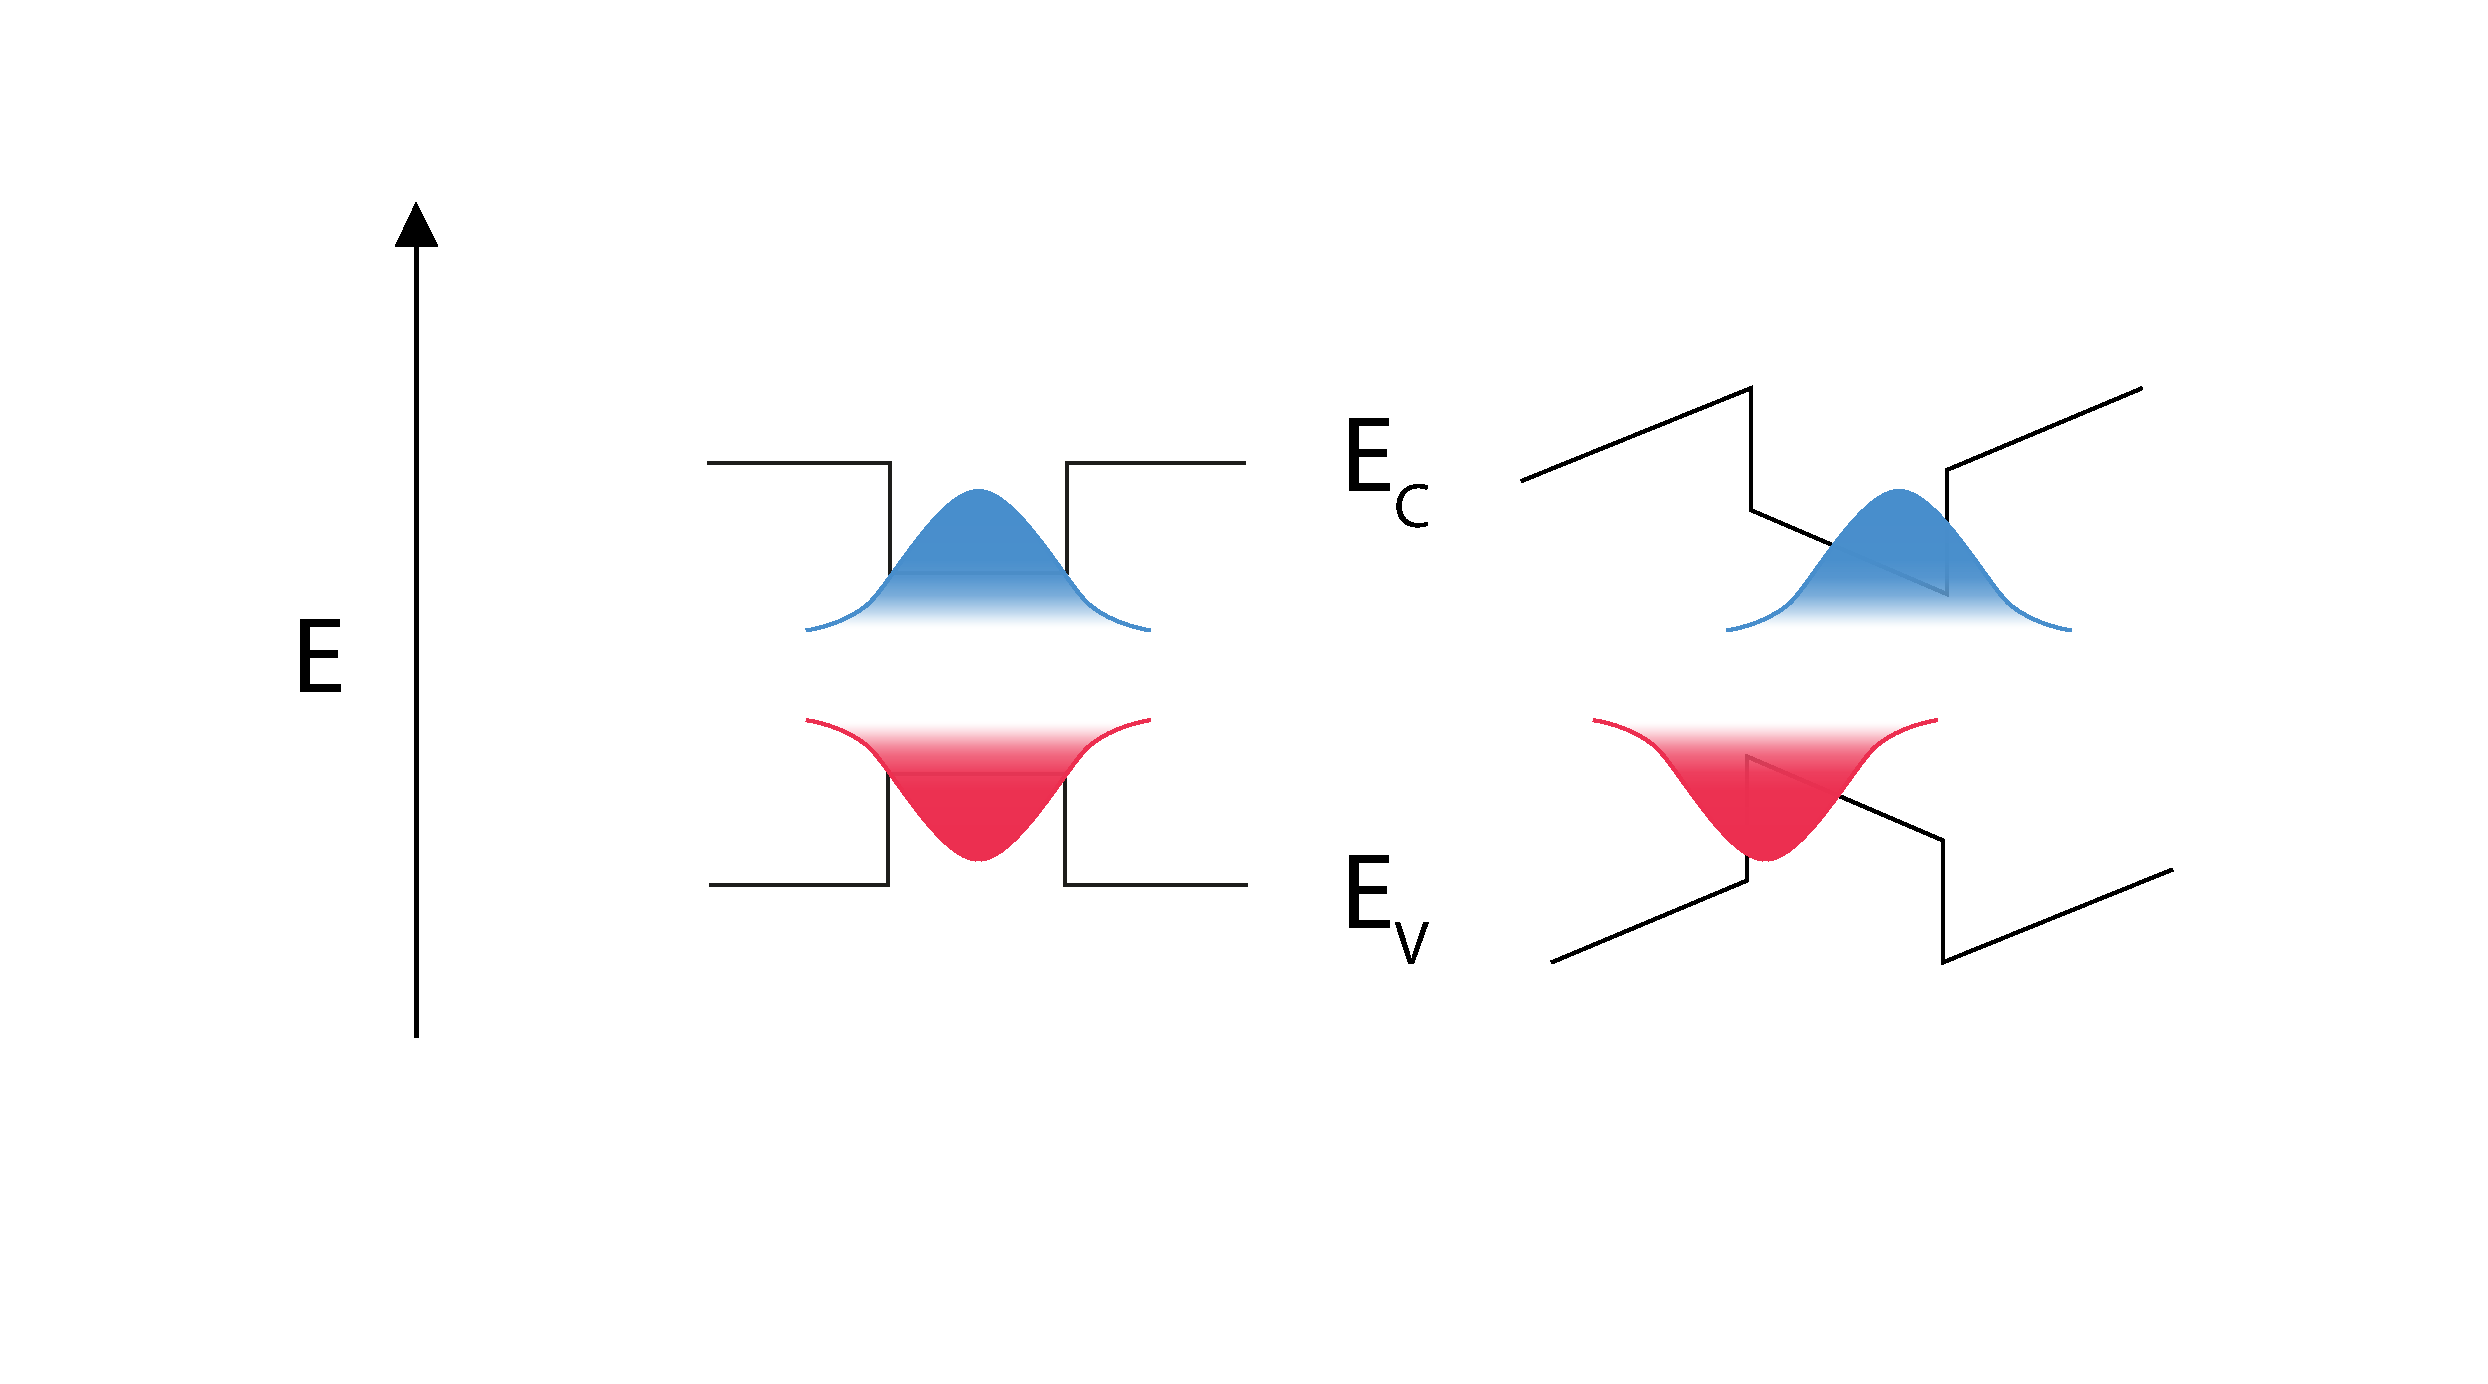
\includegraphics[width=\linewidth]{Bilder/QCSE.pdf}
        \caption{PL-Spektren der Proben ohne Übergitter}
    \end{minipage}% <- sonst wird hier ein Leerzeichen eingefügt
\end{figure}
\vspace{1cm}
\raggedright
\newpage
Die Ursache für die piezoelektrische Polarisation sind die Verspannungen zwischen den in (0001)-Richtung gewachsenen Schichten welche durch die unterschiedlichen thermischen Ausdehnungskoeffizienten und die Gitterfehlanpassung entstehen. Sie wird berechnet nach: 
%
\begin{equation}
    \vec{P}^{pz} = e \cdot \epsilon
\end{equation}
%
	
\thispagestyle{fancy}


\section{Rekombinationsmechanismen}
%
\begin{figure}[h]
\centering
\begin{minipage}[t]{1\linewidth}
\centering
\includegraphics[width=0.8\linewidth]{Bilder/bandrekomb.png}
\end{minipage}% <- sonst wird hier ein Leerzeichen eingefügt
\caption{Durch Einstrahlung eines Photons mit ausreichender Energie können Elektronen vom Valenzband in das Leitungsband angeregt werden. Von dort aus rekombinieren Elektronen und Loch entweder strahlend unter Aussendung eines Photons oder nicht-strahlend.}
 \label{fig:bandrekomb}
\end{figure}
\noindent
In der Photolumineszenzspektroskopie wird Licht als Anregungsquelle von Halbleitermaterialien für die Erzeugung eines Elektron-Loch-Paars benutzt. Dabei wird ein Elektron aus dem Valenzband in das Leitungsband angehoben und wie in Abbildung \ref{fig:bandrekomb} dargestellt ein Loch zurückgelassen. Die Elektronen relaxieren anschließend sehr schnell in das Minimum des Leitungsbandes und analog die Löcher in das Minimum des Valenzbandes. 
\newline
Leitungs- und Valenzband befinden sich im Fall von AlGaN am gleichen $\vec{k}$ -Vektor im reziproken Raum, dem sog. $\Gamma$ -Punkt. Das macht das Materialsystem AlGaN zu einem direkten Halbleiter, was von besonderem Vorteil ist. Denn ein direkter Bandübergang ist die wichtigste Grundlage für eine effiziente halbleiterbasierte Lichtquelle. 
\begin{figure}[htb]
    \centering
    \begin{minipage}[t]{0.49\linewidth}
        \centering
        \includegraphics[width=\linewidth]{Bilder/nonradRekomb.png}
        \caption{Rekombination von Elektron und Loch unter Teilnahme eines Phonons.}
				\label{fig:rekombphoton}
    \end{minipage}% <- sonst wird hier ein Leerzeichen eingefügt
    \hfill
    \begin{minipage}[t]{0.49\linewidth}
        \centering
        \includegraphics[width=\linewidth]{Bilder/radRekomb.png}
        \caption{Strahlende Rekombination von Elektron und Loch und Aussendung eines Photons}
    \end{minipage}
\end{figure}
\noindent
Die Wahrscheinlichkeit einer Anregung und daraufhin folgenden Rekombination unter Aussendung eines Photons ist deutlich höher, da kein Phonon am Prozess beteiligt sein muss (Abb. \ref{fig:rekombphoton}). Die Rekombination kann dennoch auch nicht-strahlend erfolgen, weil epitaktisch gewachsene Halbleitersstrukturen herstellungsbedingt beispielsweise nicht ohne ungewollte Dotierung durch Fremdatome, Versetzungen oder Fehlstellen an Atomgitterplätzen (Vakanzen) gewachsen werden können. Diese fungieren als sogenannte Störstellen und haben diskrete Energieniveaus. 
%
\begin{figure}[h]
    \centering
    \begin{minipage}[t]{0.75\linewidth}
        \centering
        \includegraphics[width=\linewidth]{Bilder/rekbomChannels.png}
        \caption{Übersicht über die beteiligten Rekombinationsprozesse im ABC-Modell, dabei stellt (a) die SRH-Rekombination, (b) die Auger-Rekombination und (c) die strahlende Rekombination dar.}
        \label{fig:rekombChannels}
    \end{minipage}% <- sonst wird hier ein Leerzeichen eingefügt
\end{figure}
\noindent
%
Dazu werden drei Prozesse betrachtet: Zuallererst die nichtstrahlende Rekombination, die durch die Shockley-Read-Hall- (SRH-) Rekombination an Defekten beschrieben und durch den Parameter $A$ berücksichtigt wird ($R_{nonrad} = A \cdot n $). Sie ist linear abhängig von der Ladungsträgerdichte $n$. Sie findet unter der Beteiligung eines Defektniveaus und eines Phonons statt. Der A-Koeffizient ist invers proportional zur SRH-Rekombinations-Lebensdauer. Diese wurde bei defektreichen AlGaN-Schichten im Bereich von einigen $ps$ gemessen. Mit AlGaN-QWs mit Bulk-AlN-Substraten wurden dagegen bereits Lebensdauern im Bereich einiger $ns$ erreicht \cite{1882-0786-4-9-092101} \cite{doi:10.1002/pssc.201100424}.
\newline
Der strahlende Prozess der spontanen Rekombination ist für niedrige Ladungsträgerdichten quadratisch in $n$ und tritt als Zwei-Teilchen Prozess, bei dem Loch und Elektron beteiligt sind ($R_{rad} = B \cdot n^2 $), auf. Dieser wird  mit dem Koeffizienten B beschrieben. Der B-Koeffizient ist stark abhängig vom Design des MQWs wie z.B. der QW-Dicke, QW-Barrieren-Höhe, Verzerrung des AlGaN-QWs und dem Polarisationsfeld im QW \cite{kneissl}. Typische Werte für den B-Koeffizienten liegen in einem Bereich um $2 \cdot 10^{-11} \thinspace cm^3 \thinspace s^{-1}$ \cite{1882-0786-8-2-022104} \cite{1882-0786-4-5-052101}.  
\newline
Der letzte Prozess ist die Auger-Rekombination, die speziell für sehr hohe Anregungsleistungsdichten relevant ist und dann durch die kubische Abhängigkeit stark dominiert ($R_{auger} = C \cdot n^3 $). Dabei gibt ein bereits in das Leitungsband angeregte Elektron seine Energie an ein weiteres Elektron im Leitungsband ab. Dieses relaxiert dann entweder wieder zum Leitungsbandminimum unter Mitwirkung von Phononen oder verlässt bei Oberflächennähe den Kristall. Der letzte Fall bildet die Grundlage für die Auger-Elektronen-Spektroskopie.
Die Größenordnung des C-Koeffizienten für die Gruppe-III-Materialien ist immer noch in Diskussion \cite{8b1c5cf85d5a45e0ae9acca7b03dc349} \cite{doi:10.1063/1.2785135} \cite{doi:10.1002/pssc.200880950} und die Werte für blau-violette LEDs liegen zwischen $1 \cdot 10^{-31}$ und $2 \cdot 10^{-30} \thinspace cm^6 \thinspace s^{-1}$. Die Messmethoden zur Bestimmung des C-Koeffizienten für UV-LEDs sind noch ungenauer \cite{1882-0786-8-2-022104}. Theoretische Modelle sagen aber voraus, dass der C-Koeffizient kleiner werden sollte mit kleiner werdender Wellenlänge \cite{doi:10.1063/1.3570656}.
\newline
Die effektive Rekombination ist somit die Summe aus der strahlenden Rekombination, der nicht-strahlenden Rekombination und der Auger-Rekombination.
\begin{equation}
    R_{eff} = R_{rad} + R_{nonrad} + R_{auger}
    \label{eq:iqe1}
\end{equation}
Der allgemein verwendete Ansatz zur Beschreibung der effektiven Rekombinationsrate $R_{eff}$ (oder auch Generationsrate $G$) wird mit Hilfe der genannten Koeffizienten beschrieben. Er beruht auf der Abhängigkeit der beteiligten Prozesse von der Ladungsträgerdichte $n$ und wird daher auch als ABC-Modell bezeichnet.
\begin{equation}
    R_{eff} (G) = A \cdot n + B \cdot n^2 + C \cdot n^3 
    \label{eq:iqe2}
\end{equation}
Weiter wird angenommen, dass die Anregungsleistungsdichte des Lasers P proportional zu
der Ladungsträger-Generationsrate G ist. Die strahlende Rekombination $R_{rad}$ wird hauptsächlich durch den Überlapp der Wellenfunktionen von Elektronen und Loch im Leitungsband und Valenzband des QW beeinflusst. Dieser wiederum ist stark abhängig vom QCSE (Abb. 
\ref{fig:qcse}) und besonders bedeutend bei heteroepitaktisch gewachsenen Halbleiterstrukturen. 
%

	\newpage
\section{Bestimmung der internen Quanteneffizienz}
\thispagestyle{fancy}
\begin{figure}[h]
    \centering
    \begin{minipage}[t]{0.49\linewidth}
        \centering
        \includegraphics[width=\linewidth]{Bilder/IQEohneDotierungVerschAParams.pdf}
        \caption{Abhängigkeit der internen Quanteneffizienz von der Ladungsträgerdichte für feste Parameter B und C. Der Parameter A wird mit 9 verschiedenen Werten von $0 s^{-1} $ bis $10^9 s^{-1}$ variiert ~\cite{semreich}.}
        \label{fig:abha}
    \end{minipage}
    \hfill
    \begin{minipage}[t]{0.49\linewidth}
        \centering
        \includegraphics[width=\linewidth]{Bilder/BeispielIQEbestimmen.pdf}
        \caption{Photolumineszenzspektrum bei $5K$ und $300K$. Die integrierte Intensität ist die Fläche des jeweiligen Spektrums.}
        \label{fig:beispielint}
    \end{minipage}% <- sonst wird hier ein Leerzeichen eingefügt
\end{figure}
\noindent
Die aktive Region einer idealen LED würde für jedes injizierte Elektron jeweils ein Photon aussenden. 
Das bedeutet, dass die IQE, die nach \cite{schub} wie folgt definiert ist,
\begin{equation}
    IQE = \frac{ \footnotesize \text{Anzahl der Photonen die von der aktiven Zone emittiert werden pro Sekunde}}{ \footnotesize \text{Anzahl der Elektronen die in die LED injiziert werden pro Sekunde}}
\end{equation}
den Wert $1$ annehmen müsste. Die IQE kann somit analog als Verhältnis von strahlender Rekombination und der effektiven Rekombination beschrieben werden. Ausgedrückt durch Ratengleichungen und mit \ref{eq:iqe1} ist die IQE in ihrer einfachsten Form somit
\begin{equation}
    IQE = \frac{B \cdot n^2}{A \cdot n + B \cdot n^2 + C \cdot n^3} = \frac{R_{rad}}{R_{eff}}
\end{equation}
Die IQE kann experimentell mit Hilfe der Photolumineszenzspektroskopie bestimmt werden, indem angenommen wird, dass keine thermisch aktivierten Defekte bei Tieftemperatur vorhanden sind
\begin{equation}
    A \propto e^{\frac{-E_{activation}}{kT}}
\end{equation}
Mit dieser und der Annahme, dass keine Auger Rekombination ($ C \cdot n^3 $) auftritt, ist die IQE bei Tieftemperatur ($ \propto 5K$) gleich 1. Somit kann die IQE als Quotient der integrierten PL Intensität bei Temperatur T und integrierter PL Intensität bei Tieftemperatur ($5K$) beschrieben werden.
\begin{equation}
    IQE(T) = \frac{\text{\textcolor[rgb]{0.65,0.16,0}{Integrierte PL Intensität (T)}}}{ \textcolor[rgb]{0,0,1}{\text{ Integrierte PL Intensität } (T \rightarrow 0 K)} }
    \label{eq:standardiqe}
\end{equation}
Die IQE ist folglich abhängig von der Temperatur, da der Parameter A für die SRH-Rekombination temperaturabhängig ist (Abb. \ref{fig:abha}). 
Um also die IQE bei Raumtemperatur zu bestimmen, wird das Spektrum einer Probe bei 5K und 300K bei ansonsten möglichst gleichen Bedingungen aufgenommen, wie in Abbildung \ref{fig:beispielint} exemplarisch dargestellt ist. Die Intensität in Abhängigkeit der Wellenlänge wird interpoliert, dann integriert und dann das Verhältnis berechnet. 
%
	
\section{Bestimmung der IQE bei Raumtemperatur durch Fitting}

\thispagestyle{fancy}

In diesem Kapitel soll nun eine in \cite{doi:10.1063/1.3100773} und \cite{doi:10.1063/1.4917540} gezeigte Methode zur Bestimmung der IQE durch ein Fitting-Modell für die integrierte Intensität in Abhängigkeit der Ladungsträgerdichte vorgestellt werden. Angefangen mit der Rekombinationasrate, geht das Modell davon aus,
das bei Raumtemperatur Auger-Rekombination nur bei sehr hohen Anregungsleistungsdichten Relevant ist, wegen der kubischen Abhängigkeit der Auger-Rekombination von der Ladungsträgerdichte $n$
\begin{equation}
    G = R_{eff} = A \cdot n + B \cdot n^2
\end{equation}    
G steht hierbei für Generationsrate und beschreibt namentlich die Rate der Ladungsträger die durch Bestrahlung mit dem Laser erzeugt werden und entspricht hierbei der effektiven Rekombinationsrate $R_{eff}$



	\thispagestyle{fancy}

\section{Optische Polarisation und Valenzbandstuktur}
%
\begin{figure}[ht]
    \centering
    \begin{minipage}[t]{0.49\linewidth}
        \centering
        \includegraphics[width=\linewidth]{Bilder/vancebandPlot.png}
        \caption{Die energetische Reihenfolge der Valenzbänder in Abhängigkeit der Kristallfeldaufspaltung. Sichtbar ist der Wechsel der Bandanordnung mit sinkender Kristallfeldaufspaltung und der Effekt des "`anti-crossing"' bei den Bändern gleicher Symmetrie.    }
        \label{fig:auger5k}
    \end{minipage}% <- sonst wird hier ein Leerzeichen eingefügt
    \hfill
    \begin{minipage}[t]{0.49\linewidth}
        \centering
        \includegraphics[width=\linewidth]{Bilder/martinTETM.png}
        \caption{Die Grafik zeigt die sich kontinuierlich ändernde Abstrahlcharakteristik in Abhängigkeit der Polarisation von TE- zu TM~\cite{martingut}.  }
        \label{fig:trueiqe}
    \end{minipage}
\end{figure}
\vspace{0.1cm}
\raggedright
Durch die Prozessierung und die Flip-Chip-Montage kann Licht nur durch die untere, unbewachsene Seite des Saphir-Substrates ausgekoppelt werden. Die Art und Weise der Lichtauskopplung hat einen bedeutenden Einfluss auf die Extraktionseffizienz und damit auf die externe Quantenffizienz(EQE). Durch die Geometrie bestimmt, hängt die Extraktionseffizienz maßgeblich vom Emissionsprofil ab, so dass Licht welches senkrecht zur Quantenfilmebene abgestrahlt wird, die höchste Extraktionseffizienz aufweist. 
Um diese zu optimieren, ist es wichtig die Bandstrukturen zu betrachten.
\newline
Die Valenzbandstrukturen von AlN und GaN unterscheiden sich durch die unterschiedliche anordnung der Bänder. Neben dem Leitungsband gibt es ein durch Spin-Bahn-Wechselwirkung und Kristallfeldenergie dreifach aufgespaltenes Valenzband~\cite{doi:10.1063/1.117689}. Sie werden nach ihrer energetischen Lage als A-,B- und C-Band bezeichnet. In AlN hat das A-Band eine $\Gamma^{L}_{7+}$, das B-Band eine $\Gamma^{L}_{9}$ und das C-Band eine $\Gamma^{L}_{7}$ Symmetrie. Bei GaN hingegen gilt folgende Reihgenfolge:  $\Gamma^{L}_{9}$, $\Gamma^{L}_{7+}$, $\Gamma^{L}_{7}$. Die Ursache für den Symmetriewechsel liegt in der großen negativen Kristallfeldenergie von AlN mit einem Wert von $-221meV$ \cite{PhysRevB.87.235209} im Vergleich zur positiven von GaN mit $12,3meV$ ~\cite{PhysRevB.81.155202}. Bei Raumtemperatur wird, nach der Fermi-Dirac-Verteilung, das oberste Band mit der $\Gamma^{L}_{7+}$-Symmetrie, besetzt und aus Zuständen des $p_z$ bestehend, wird transversal magnetisch (TM) polarisiertes Licht emittiert ist. Die strahlende Rekombination findet demnach überwiegend mit Elektronen und Löchern aus dem A-Band mit $\Gamma^{L}_{7+}$-Symmetrie statt.
In GaN ist das oberste Valenzband am $\gamma$-Punkt mit $\Gamma^{L}_{9}$-Symmetrie . Das elektrische Feld des Lichtes ist senkrecht zur c-Kristallachse und wird durch Übergänge ins A- und B- Band erzeugt~\cite{doi:10.1063/1.3574025}, die aus Zuständen des $p_x$-und $p_y$-Orbitals bestehen. Bei strahlender Rekombination von Elektronen mit den Löchern im A- und B-Band entsteht also überwiegend TE-polarisiertes Licht ~\cite{doi:10.1063/1.3574025} . 
TM polarisiertes Licht kann nicht ausgekoppelt werden, da es nur in der x-y- Ebene (parallel zur Quantenfilmebene) emittiert. Daraus resultierend sinkt die Extraktionseffizienz und damit die EQE. Bei $Al_{x}Ga_{1-x}N$ kommt es mit steigendem Aluminiumgehalt zu einer kontinuierlichen Verschiebung der Valenzbänder und es kommt zum sog. "`anti-crossing"' des $\Gamma^{L}_{7+}$ und $\Gamma^{L}_{7-}$ und resultiert in einer Änderung der Oszillatorstärke und damit der Polarisationseigenschaften ~\cite{doi:10.1063/1.4932651}.  Bedeutet, die Lichtemission ändert sich von hauptsächlich TE-polarisiertem Licht zu TM-polarisiertem Licht. Der genaue Aluminiumgehalt, an dem die Valenzbandkreuzung auftritt, ist noch nicht hinreichend bekannt. Theoretische Betrachtungen sagen für unverzerrtes $Al_{x}Ga_{1-x}N$ einen Kreuzungspunkt bei ca. $7\%$ vorher ~\cite{doi:10.1063/1.3675451}. Durch den starken Einfluss von Verzerrungen auf die Energie der  Valenzbandkante, ist die Polarisation abhängig von der wachsenden biaxialen Verzerrung bei steigendem Aluminiumgehalt. So wurde von Kawanishi et al. experimentell der Wechsel bei einem Aluminiumgehalt von "`75\%"' festgestellt ~\cite{doi:10.1063/1.2410242}. Noch dazu ist ist die Polarisation bei Mehrfachquantenfilmen(engl. multiple quantum wells, kurz MQW) abhängig vom Ladungsträgereinschluss (engl. quantum confinement). Dieser ist hauptsächlich bestimmt durch die Barrierenhöhe und Barrierendicke. Mit kleiner werdender Barrierendicke, steigt der Grad der Polarisation durch den gesteigerten Einfluss des QCSE ~\cite{PhysRevB.84.035305}. 
\newline
\begin{figure}[ht]
    \centering
    \begin{minipage}[t]{0.49\linewidth}
        \centering
        \includegraphics[width=\linewidth]{Bilder/christophPolarisationSimu.png}
        \caption{Simulationsergebnisse des Polarisationsgrades in Abhängigkeit der Aluminiumkonzentration der Barrieren und Quantentöpfe, basierend auf
dem k·p-Modell, für AlGaN-QW mit $1.5nm$-Dicke, die pseudomorph auf ELO-AlN gewachsen wurden. Die gestrichelte Linie zeigt, dass der Wechsel der Polarisation abhängig ist vom Aluminiumanteil in den Barrieren und QWs ~\cite{doi:10.1063/1.4932651} .  }
        \label{fig:simuchr}
    \end{minipage}% <- sonst wird hier ein Leerzeichen eingefügt
    \hfill
    \begin{minipage}[t]{0.49\linewidth}
        \centering
        \includegraphics[width=\linewidth]{Bilder/christophPolarisationSimu1.png}
        \caption{ Ergebnisse der Simulation für die Polarisation in Abhängigkeit von der QW-Dicke(Wellenlänge) und dem Al-Gehalt in den QWs ~\cite{doi:10.1063/1.4932651} .  }
        \label{fig:simu1chr}
    \end{minipage}
\end{figure}
\vspace{0.1cm}
\raggedright
Reich et al. untersuchte unter diesem Zusammenhang die optische Polarisation der Emission von UVC-Leuchtdioden(LEDs) auf Basis von (0001) orientierten $Al_{x}Ga_{1-x}N$-MQWs mit Simulationen und Elektrolumineszenzmessungen ~\cite{doi:10.1063/1.4932651}. Dabei stellte er fest, dass mit zunehmendem Aluminium-Gehalt in den QWs die inplanare-Intensität des TE polarisierten Lichtes gegenüber dem des TM polarisierten Lichts abnimmt, was auf eine Neuordnung der Valenzbänder in $Al_{x}Ga_{1-x}N$ zurückzuführen ist. 
Durch Modellrechnungen, basierend auf dem k·p-Modell, wurde das Design der aktiven Zone von AlGaN MQWs optimiert, wodurch eine erhöhte TE-Polarisation und damit eine höhere Extraktionseffizenz für bottom-emitting LEDs im tiefen UV-Spektralbereich ergibt. Unter der Annahme von schmalen Quantentöpfen, Barrieren mit hohem Aluminium-Gehalt und voll verspanntem Wachstum auf AlGaN-Bulk Substraten wurde bei einer Wellenlänge von nur $239 nm$ eine starke TE-polarisierte Emission beobachtet.
Mit Hilfe der Photolumineszenz lässt sich die Polarisation ebenfalls bestimmen, in dem die Polarisation $\rho$ der Photolumineszenzemission aus der Kante einer Probe mit Hilfe der Gleichung 
\begin{equation}
\rho = \frac{ I_{TE} - I_{TM} }{ I_{TE} - I_{TM} } 
\end{equation}
bestimmt wird. Dabei ist $I_{TE}$ die integrierte Intensität der TE-polarisierten und $T_{TM}$ die Intensität der TM-polarisierten Emission. 
 


	
\chapter{Aufbau}


\thispagestyle{fancy}

\section{Photolumineszenzaufbau}

Für die experimentelle Untersuchung der UV-Photolumineszenz wurde der PL-Aufbau der AG-Kneissl verwendet, den Christoph Reich in der Zeit seiner Masterarbeit aufgebaut und während seiner Promotion erweitert hat~\cite{creich}. 
Als Anregungsquelle für die Photolumineszenz dient ein ArF-Excimerlaser mit einer Wellenlänge von $193 \ nm$ ($6,4 \ eV$). Mit dieser Wellenlänge ist er bestens geeignet für die Überbandanregung von Nitridhalbleitern. 
Des Weiteren bietet der Aufbau die Möglichkeit von temperaturabhängigen Untersuchungen von $5 \ K $ bis $300 K$. Dies ist auch die Grundlage für die Bestimmung der Internen Quanteneffizienz (kurz IQE), die den Großteil der Thematik dieser Arbeit ausmachen wird. 
\newline
Der Laser mit dem Modellnamen  "Xantos" von der Firma Coherent bietet eine maximale Emissionsenergie von $ 5 \ mJ $ und die Frequenz ist bis zu 500 Hz einstellbar bei einer Pulsdauer von $5 \ ns$. 
Durch interne Rückkopplung ist eine Energiestabilisierung möglich, die die Schwankung der Anregungsleistung auf 3 Prozent minimiert. 
\newline
Die Ansteuerung des kompletten Messvorgangs erfolgt durch die Messsoftware von Christoph Reich, entwickelt in der grafischen Programmiersprache "LabView" von Texas Instruments. Mit dieser ist es möglich alle nötigen Einstellungen an Pumpen, Heizern, Laser, Filtern und Spektrometer vorzunehmen, um einen komplett automatisierten Messvorgang zu starten, der nur noch aus Sicherheitsbedingungen überwacht werden muss. Spektren können so mit verschiedenen Parametern wie Position, Anregungsleistungsdichte, Temperatur, Energiebereich und Integrationszeit aufgenommen werden und auch ein Gaswechsel ist möglich.
\newline
Beginnend vom Laser wird im ersten Schritt der Lasterstrahl durch ein Linsensystem bestehend aus einer Zerstreuungs- und Sammellinse aufgeweitet. Dieser Schritt ermöglicht es, die Anregungsleistungsdichte zu verringern, um die am Aufbau beteiligten Gerätschaften nicht mit zu hohen Leistungen zu beschädigen. Damit sind insbesondere die Filterräder gemeint. Mit Hilfe der Filterräder ist es möglich, die Anregungsleistungsdichte 61 stufig zu variieren und somit leistungsdichteabhängige IQE Messungen zu machen. Als nächstes passiert der Strahl ein Linsensystem aus zwei Sammellinsen für eine Strahlverkleinerung. Vor dem Auftreffen des Strahles am Probenhalter im Kryostaten passiert der Strahl noch eine Lochblende. Sie dient der Entfernung achsennaher Strahlen und um bei Bedarf den Strahldruchmesser noch weiter zu verringern. Um den Strahl in Richtung des Probenhalters durch das Fenster im Kryostaten zu lenken, wird ein Spiegel mit einer dielektrischen Beschichtung benutzt. Der Laserstrahl durchdringt die Fenster des Kryostaten, diese sind speziell für eine hohe Transmission in diesem Wellenlängenbereich ausgelegt. Der Kryostat selbst ist horizontal und vertikal verfahrbar um die Messung mehrerer Proben im Probenhalter in einem Vorgang zu ermöglichen. Die Proben werden mit einem Kleber auf dem Probenhalter selbst befestigt, bevor dieser in den Kryostaten geschoben wird. 
Die Anregung der Proben mit dem Laserstrahl führt zur Proben spezifischen Emission von Licht. Diese wird von einer Linse im Strahlengang vor dem Detektor eingefangen und von einer zweiten Linse eingefangen die auf den Monochromatorspalt fokussiert ist.


	
\thispagestyle{fancy}

\section{Bestimmung der Degradation des UV Quarzglases}
%
\begin{figure}[htb]
  \centering
  \begin{minipage}[t]{0.49\linewidth}
      \centering
      \includegraphics[width=\linewidth]{Bilder/uvsilicaDegradation.png}
      \caption{Vom Hersteller angegebene wellenlängenabhängige Transmission vor und nach Degradation durch Bestrahlung.}
      \label{fig:degra}
  \end{minipage}
\end{figure}
\noindent
Da die Messung der Anregungsleistungdichte erfolgt, bevor das Laserlicht die Probe durch das UV-Quarzglas im Kryostaten trifft, ist es wichtig den Transmissionsverlust zu bestimmen, um die realen Werte für die Anregungsleistungsdichte zu kennen (Die Anregungsleistungsdichte, die bei der Probe ankommt). Der Kryostat besitzt vier Fenster, bestehend aus UV-Quarzglas, das besonders transparent im UV-Wellenlängenbereich ist. Durch diese Fenster dringt das Laserlicht in den Probenhalter ein. Von diesen Fenstern war und ist eines in dauerhaftem Gebrauch. Wie in Abbildung \ref{fig:degra} zu sehen ist, weisen die Fenster aber mit der fortlaufender Bestrahlung Degradation auf. So nimmt laut Hersteller durch Degradation die Transmission von 90 Prozent bis auf ca. 75 Prozent für eine Wellenlänge von 193 nm ab.
\newline
Um nun den Transmissongrad zu bestimmen, wurde der Probenhalter aus dem Kryostat entfernt, damit das Laserlicht ungehindert durch zwei parallel liegende Fenster durchdringen kann, um so auch die Anregungsleistungsdichte des Laserlichtes nach durchdringen des letzten Fenster messen zu können. So konnte die Anregungsleistungsdichte vor dem Eintreten und nach dem Austreten in den Kryostaten bestimmt werden. 
\newline
Dies wurde einmal bei den parallel liegenden unbenutzten Fenstern durchgeführt. Davon ausgehend, dass beide Fenster, da unbenutzt, den gleichen Transmissionsgrad haben, kann darauf zurückgeschlossen werden, dass ein unbenutztes Fenster einen Transmissionsgrad von 59 Prozent aufweist. Dies weicht um ca. 10 Prozent von der Herstellerangabe ab, die aber nicht die Reflektion im Kryostaten miteinbezieht. 
%
\begin{figure}[htb]
  \centering
  \begin{subfigure}{0.40\textwidth}
    \centering
    \includegraphics[width=0.9\linewidth]{Bilder/uvsilicavergleich.pdf}
    \caption{PL Intensität in Abhängigkeit der Anregungsleistungsdichte mit den benutzten und unbenutzten Fenstern}
    \label{fig:sub1}
  \end{subfigure}%
  {\LARGE$\xrightarrow{\cdot 0,44}$}
  \begin{subfigure}{0.40\textwidth}
    \centering
    \includegraphics[width=0.9\linewidth]{Bilder/uvsilicaVergleichSkaliert.pdf}
    \caption{Die Anregungsleistungsdichte des unbenutzten Fensters mit den rechnerisch bestimmten 0,44 skaliert}
    \label{fig:sub2}
  \end{subfigure}
  \caption{}
  \label{fig:vergleichSkaliert}
\end{figure}
\newline
Um den Transmissionsgrad des benutzten Fensters zu bestimmen, wurde die Transmission durch das benutzte und dem parallel liegende unbenutzte Fenster gemessen. Mit dem Wissen, dass der Transmissionsgrad durch das unbenutzte Fenster bei 59 Prozent ($T_{unb} = 0,59$) liegt, kann die Transmission durch das benutzte Fenster auf 26 Prozent ($T_{ben} = 0,26$) berechnet werden. 
Davon ausgehend, dass die Transmission bei höheren Wellenlängen (Emission) gleich und bei beiden Fenstern ähnlich ist,
%
\begin{equation}
  F_{skal} = \frac{ T_{ben} }{ T_{unb} } = 0,44\label{eq11}
\end{equation}
%
kann der Skalierungsfaktor mit für die Anregungsleistungsdichte auf 0.44 bestimmt werden. Dies bedeutet, dass durch Degradation die Transmission auf 44 Prozent der ursprünglichen Transmission gesunken ist.
\newline
Dies bestätigt sich auch durch die Gegenüberstellung in  Abbildung \ref{fig:vergleichSkaliert}. Somit ist durch die zeitliche Degradation die Transmission auf 44 Prozent der ursprünglichen gesunken. Dies bestätigt im Umkehrschluss, dass von der ausgehenden Anregungsleistungsdichte, die vor dem Kryostaten gemessen wird, durch die geringe Transmission der Fenster und Reflektion im und außerhalb des Kryostaten nur ca. 26 Prozent des vom Laser emittierten Lichtes bei der Probe ankommen. 
	\section{Aufbau: Erweiterung der Filterkombinationen}
\thispagestyle{fancy}

Im Zuge dieser Arbeit wurden für eine Erhöhung der Messpunkte und Verringerung von Rauschen bei der leistungsdichteabhängigen Messung der IQE die Anzahl der Filterkombination erhöht. Dafür wurden die alten zwei Filterräder durch drei neue ersetzt. 
%
\begin{figure}[ht!]
    \centering
    \begin{minipage}[t]{1\linewidth}
        \centering
        \includegraphics[width = 0.49\linewidth]{Bilder/AuswertungNovemeberKorr1VergleichFilter.pdf}
        \caption{Vergleich der Messung von insgesamt 5 ähnlichen Proben. 3 Proben (blau) wurden mit dem alten Setup gemessen. 2 Proben (grün, durchgezogene Linie) wurden mit dem neuen Setup gemessen. Die Präzision in tieferen Anregungsleistungsdichtenbereichen ist für das neue Setup deutlich erhöht. Das Rauschen fällt ebenfalls deutlich geringer aus. }
        \label{fig:vergleichFilter}
    \end{minipage}
\end{figure}
%
\newpage
Durch die erhöhte Anzahl möglicher Filterkombinationen ist es möglich, statt nur 27 verschiedene Messpunkte 61 zu nehmen. Speziell der Bereich der geringen Anregungsleistungsdichten kann so besser aufgelöst werden und das Rauschen wurde im Allgemeinen stark verringert \ref{fig:vergleichFilter}. 
%

	\newpage

\section{Einfluss der Auger-Rekombination auf die IQE}
%
\begin{figure}[h]
    \centering
    \begin{minipage}[t]{0.49\linewidth}
        \centering
        \includegraphics[width=\linewidth]{Bilder/AugerBei5K.pdf}
        \caption{Die Grafik zeigt die Abhängigkeit der internen Quanteneffizienz von der Ladungsträgerdichte für feste Paramater B und C unter Variation des A Parameters und Beachtung des Einflusses einer Silizium-Dotierung.}
        \label{fig:auger5k}
    \end{minipage}% <- sonst wird hier ein Leerzeichen eingefügt
    \hfill
    \begin{minipage}[t]{0.49\linewidth}
        \centering
        \includegraphics[width=\linewidth]{Bilder/NormierteKorrgierteIQE5K.pdf}
        \caption{Die Grafik zeigt die normierte korrigierte IQE bei 5K nach Gleichung [\ref{eq:iqetrue5k}] }
        \label{fig:trueiqe}
    \end{minipage}
\end{figure}
\vspace{1cm}
\raggedright
Das bisher benutzte Modell zur Bestimmung der PL-IQE ging davon aus, dass bei Tieftemperatur keine Auger-Rekombination (Gleichung) vorkommt, aber wie in Abb. [\ref{fig:auger5k}] deutlich zu erkennen, nimmt der Verlauf der PL-Intensität in doppeltlogarithmischer Darstellung gegenüber der Anregungsleistungsdichte (die direkt proportional zur Ladungsträgerdichte ist), im Bereich höherer Anregungsleistungen (entsprechend höheren Ladungsträgerdichten) deutlich ab und weist keinen linearen Verlauf mehr auf, den er aber durch eine allein quadratische Abhängigkeit (in doppeltlogarithmischer Darstellung linear) haben sollte. Dies zeigt, dass die IQE nicht, wie bisher angenommen, immer bei 100 Prozent liegt, sondern auch bei Tieftemperatur Anregungsleistungsdichte abhängig ist. Um dies zu berücksichtigen, wird nun die IQE bei 5K definiert als:
%
\begin{equation}
    IQE_{true}(T = 5K, A_{exc}) = \frac{ \frac{I_{pl}(T,A_{exc}) }{A_{exc} } } { \lvert \lvert \frac{I_{pl}(T,A_{exc})}{A_{exc}} \lvert \lvert_{max} }
    \label{eq:iqetrue5k}
\end{equation}
%
Wobei $I_{pl}(A_{exc})$ die von der Anrengungsleistungsdichte $A_{exc}$ und Temperatur $T = 5K$ abhängige integrierte PL-Intensität ist. Die integrierte PL-Intensität wird durch die Anregungsleistungsdichte dividiert und auf das Maxmimum normiert, so dass das Maximum der IQE bei $5K$ bei der geringsten Anregungsleistungdichte mit der geringsten Auger-Rekombination liegen sollte. Um nun die IQE bei Raumtemperatur zu bestimmen, wird die nach dem alten Verfahren ermittelte IQE multipliziert mit den neu ermittelten Werten passend zur Anregungsleistungsdichte. 
%
\begin{equation}
    IQE(T, A_{exc}) = \frac{IQE(T,A_{exc})}{IQE(5K,A_{exc})} \cdot IQE_{true}(5K,A_{exc})
\end{equation}
%
Die IQE bei $5K$ dient hierbei also als Skalierungsfaktor, der den Einfluss der Auger-Rekombination bei Raumtemperatur korrigiert. Somit fällt im Vergleich insbesondere auf, dass die Skalierung bei den kleinsten Anregungsleistungsdichten am geringsten Einfluss hat und mit steigender Anregungsleistungsdichte kubisch steigt, so dass die nach dem alten Verfahren ermittelten IQE-Werte bei höheren Anregungsleistungsdichten deutlich nach unten korrigiert werden müssen. 
%
\begin{figure}[h]
    \centering
    \begin{minipage}[t]{0.49\linewidth}
        \centering
        \includegraphics[width=\linewidth]{Bilder/StandardIQE300K.pdf}
        \caption{Die Grafik zeigt die Abhängigkeit der internen Quanteneffizienz von der Ladungsträgerdichte für feste Paramater B und C unter Variation des A Parameters und Beachtung des Einflusses einer Silizium-Dotierung.}
        \label{fig:standiqe300k}
    \end{minipage}% <- sonst wird hier ein Leerzeichen eingefügt
    \hfill
    \begin{minipage}[t]{0.49\linewidth}
        \centering
        \includegraphics[width=\linewidth]{Bilder/KorrigierteIQE300K.pdf}
        \caption{Die Grafik zeigt die normierte korrigierte IQE bei 5K nach Gleichung [\ref{eq:iqetrue5k}] }
        \label{fig:trueiqe300k}
    \end{minipage}
\end{figure}
\vspace{1cm}
\raggedright
%
fssfsdf

	
	\section{Einfluss der Siliziumdotierung auf die IQE}
\thispagestyle{fancy}
%
Das ABC-Modell stellt aber nur eine Vereinfachung dar und berücksichtigt nicht alle vorkommenden Effekte wie beispielsweise Lokalisierung, Screening durch Ladungsträger und Dotierung. 
Der Effekt der Dotierung spielt dabei eine besonders wichtige Rolle, da eine Silizumdotierung üblich in UV-Leds ist und einen großen Einfluss hat.
Nach \cite{schub} kann gezeigt werden, dass die Ratengleichungen, mit der Annahme einer Dotierung für die 
die Radiative Rekombination sich ändert und soll nun hergeleitet werden:
\\newline
Jeder dotierte oder undotiere Halbleiter hat zwei Arten von Ladungsträgern, Elektronen und Löcher.
Im Gleichgewicht, bedeutet ohne externe Anregung durch Absorption von Licht oder Injektion von Elektronen, ist das Produkt von Elektronen- und Lochkonzentration eine konstante Größe.
\begin{equation}
    n_0 \cdot p_0 = n_i^2
    \label{eq:constant}
\end{equation}
Hierbei sind $n_0$ und $p_0$ die Elektron- und Lochkonzentration unter Gleichgewichtsbedingung und $n_{i}$ damit die intrinsische Ladungsträgerkonzentration.
Werden zusätzlich die durch Anregung erzeugten Ladungsträger betrachtet, so ist die Gesamtladungsträgerkonzentration gegeben als Summe der Anregungs- und Gleichgewichtsladungsträger. 
\begin{equation}
    n_{ges} = n_0 + n \medspace \text{und} \medspace  p_{ges} = p_0 +  n 
\end{equation}
Hierbei sind $ n$ und $p$ die Anregungsladungsträger. 
Die Anzahl der stattfindenden Rekombination zwischen Elektronen und Löchern sind direkt proportional zur Elektronen-und Ladungsträgerkonzentration, so gilt, $R \propto n \cdot p $. Mit einer Proportionalitätkonstante, wird Rekombinationrate pro Zeit und Volumen definiert als
\begin{equation}
    R = - \frac{dn_{ges}}{dt} = - \frac{dp_{ges}}{dt} = B \cdot n_{ges} \cdot p_{ges}
\end{equation}
Weil Elektronen und Löcher bei Anregung paarweise erzeugt werden und verschwinden (durch Rekombination), gilt
\begin{equation}
    \label{eq:gleich}
    n(t) =  p(t)
\end{equation}
Die radiative Rekombinationrate wird dann mit $p_{0} = 0$ und Gleichung [\ref{eq:gleich}] zu
\begin{align}
\begin{split}
    R_{rad} &= B \cdot (n_0 + n)  \cdot (p_0 + p) ,
    \\
    R_{rad} &= B \cdot (n_0 + n) \cdot (n) ,
    \\
    R_{rad} &= B \cdot n^2 \cdot n \cdot n_0
\end{split}
\end{align}
Dabei beschreibt $n_{0}$ die Ladungsträgerkonzentration durch die Silizumdotierung. 
Somit wird die IQE zu:
\begin{equation}
    IQE = \frac{B \cdot n^2 + B \cdot n \cdot n_{0}}{A \cdot n + B \cdot n^2  + B \cdot n \cdot n_{0}+ C \cdot n^3} 
    \label{eq:dopediqe}
\end{equation}
Und hat einen enormen Einfluss auf die Ordinate, wie in Abb. [\ref{fig:abha1}] zu sehen ist.
%


	\thispagestyle{fancy}

\section{Untersuchung der optischen Polarisation an AlGaN MQWs mit Photolumineszenzspektroskopie}

Um die Polarisation und den Kreuzungspunkt der Simulationen von Christoph Reich experimentell zu \"uberpr\"ufen, wurden die Polarisation von zwei Probenserien mit Hilfe von Photolumineszenz-Spektroskopie untersucht. Die untersuchten Probenserien unterteilen sich in eine QW-Dicken-Variation (Serie A) und einer Serie mit Variation des Al-Gehalts (Serie B) in den QWs. 

\subsection{Variation des Al-Gehalts in den QWs}

Die Untersuchung der Al-Variations Serie, dient dem Zweck, anhand eines variierenden Al-Gehalts in den QWs und einem festen Al-Gehalt in der Barriere den \"Ubergang von TE zu TM (siehe Abb. [\ref{fig:simuchr}] in Kapitel \ref{chap:polgrund}) bei fester QW-Dicke experimentell zu \"uberpr\"ufen. Dazu wurden vier Proben auf ELO-AlN gewachsen, mit einer darauf folgenden AlN(100\%) Buffer-Schicht. Auf die Buffer-Schicht folgt zuletzt die aktiven Zone, mit einem zwischen der ersten und letzten undotierten AlN-Barriere eingebetteten dreifach $Al_{x}Ga_{1-x}N$ QWs mit einer Dicke von $1,5nm$ und dazwischen AlN-Barrieren einer Dicke von $5nm$. Der Aluminium-Gehalt der QWs wurde variiert mit x= 60 \%, 68 \%, 73 \%, 81 \%. 
Der Einfluss des unterschiedlichen Al-Gehalts auf die Emissionsenergie ist in Abb. [\ref{fig:alvariationSpektrum}] zu erkennen. Die kleinste Wellenl\"ange hat Probe A:4 mit einem Al-Gehalt von $81\%$, die theoretisch ausreicht um im Vergleich mit den anderen Proben zumindest einen Abfall des Polarisationgrades der TE-Polarisation zu erkennen.
%
\begin{figure}[htb]
  \centering
  \begin{minipage}[t]{0.49\textwidth}
    \centering
    \includegraphics[width=\textwidth]{Bilder/spektrenAlvariation.pdf}
    \caption{PL-Spektren der Serie A. Die Emission verschiebt sich mit steigendem Al-Gehalt in den QWs hin zu kleineren Wellenl\"angen durch die steigende Bandl\"uckenenergie.  }
    \label{fig:alvariationSpektrum}
  \end{minipage}
	\hfill
  \begin{minipage}[t]{0.49\textwidth}
    \centering
    \includegraphics[width=\linewidth]{Bilder/polarisationAlvariation.pdf}
    \caption{PL-Spektren der Serie A. Die Emission verschiebt sich mit steigendem Al-Gehalt in den QWs hin zu kleineren Wellenl\"angen durch die steigende Bandl\"uckenenergie. }
    \label{fig:alvariationPolarisation}
  \end{minipage}
\end{figure}
%
Die Proben wurde alle bei Raumtemperatur (300K) untersucht und die Emission wurde aus der Kante der Probe gemessen um eine Absorption und Einfluss an der obersten Barriere zu vermeiden. Weil es m\"oglicherweise Auswirkungen des ELO auf die Polarisation gibt, wurde der Einfluss des ELO mit untersucht. 
Dazu wurden Proben vertikal und horizontal zur ELO-Richtung positioniert und gemessen. Abbildung [\ref{fig:alvariationPolarisation}] zeigt die Ergebnisse der Polarisationsmessungen. So zeigen die Proben A:1 und A:2 mit einem Al-Gehalt von $60\%$ und $68\%$ TE-Polarisation. Der Grad der Polarisation ist zus\"atzlich noch abh\"angig von der Positionierung der ELO-Streifen. So haben die Proben A:1 und A:2 vertikal zur ELO-Richtung Polarisationsgrade von $\rho = 0,33$ und $\rho = 0,30$ und parallel zur ELO-Richtung deutlich geringe Polarisationsgrade mit $\rho = 0,22$ und $\rho = 0,25$. Die Proben A:3 und A:4 mit $73\%$ und $81\%$ Al-Gehalt weisen TM-Polarisation auf mit Polarisationsgraden von $\rho = -0,09$ und $\rho = -0,05$ vertikal zur ELO-Richtung und $\rho = -0,11$ und $\rho = -0,14$ parallel zur ELO-Richtung. Es zeigt sich demzufolge, dass die Polarisation sich mit steigendem Al-Gehalt von TE- hin zu TM-Polarisation \"andert durch die Neuordnung der Valenzb\"ander. Der Wechsel findet bei einer Wellenl\"ange von ca. $240nm$ statt und ist in guter \"Ubereinstimmung mit den Simulation (siehe Abb. [\ref{fig:simuchr}]). \"Uberdies ist eine Abh\"angigkeit der Ausrichtung der ELO-Streifen zu beobachten. M\"ogliche Erkl\"arungen w\"aren, dass es durch Brechungsindexwechsel vom Freiraum des ELO zum Kristall, es zu Reflektion des emittierten Lichtes und damit zu Interferenzerscheinungen kommen k\"onnte oder das ELO beeinflusst die Verzerrung im Kristall so, dass die f\"ur die Simulation angenommene biaxiale Verzerrung nicht mehr zutrifft. 

\subsection{Variation der QW-Dicke}

Die Untersuchung der QW-Dicken Variations Serie, dient dem Zweck, anhand der variierenden QW-Dicke bei einem festen Al-Gehalt in QW und Barriere den \"Ubergang von TE zu TM (siehe Abb. [\ref{fig:simu1chr}] in Kapitel \ref{chap:polgrund}) experimentell zu \"uberpr\"ufen. Dazu wurden vier Proben auf ELO-AlN gewachsen, mit einer darauf folgenden AlN(100\%) Buffer-Schicht. Auf die Buffer-Schicht folgt zuletzt die aktiven Zone, mit einem zwischen der ersten und letzten undotierten AlN-Barriere eingebetteten dreifach $Al_{0.6}Ga_{0.4}N$ QWs und dazwischen $Al_{0.81}Ga_{0.19}N$-Barrieren einer Dicke von $5nm$. Der QW-Dicke $d$ wurde variiert mit d . 
Der Einfluss des unterschiedlichen Al-Gehalts auf die Emissionsenergie ist in Abb. [\ref{fig:alvariationSpektrum}] zu erkennen. Die kleinste Wellenl\"ange hat Probe A:4 mit einem Al-Gehalt von $81\%$, die theoretisch ausreicht um im Vergleich mit den anderen Proben zumindest einen Abfall des Polarisationgrades der TE-Polarisation zu erkennen.
	\chapter{Ergebnisse}
\thispagestyle{fancy}
\section{Untersuchung optisch gepumpter Laserstrukturen auf unterschiedlichen Templates}


Dieses Kapitel widmet sich der Untersuchung der beiden Probenreihen TS4045 und TS4048 von optisch gepumpten Laserstrukturen die aus Rezepten aus zwei unterschiedlichen Serien stammen. Die beiden Serien unterscheiden sich im wesentlichen dadurch, dass sie mit(TS4048) und ohne Übergitter(TS4045) gewachsen wurden. Jede Reihe für sich weist  zusätzlich noch Unterschiede den Proben selbst auf, so sind zwei Proben der Reihe TS4045 auf AlN-Bulk zweier unterschiedlicher Hersteller (HexaTech, IKZ) gewachsen und alle  anderen Proben auf ELO AlN/Sapphire mit jeweils 3 unterschiedlichen "offcut"-Winkeln. Tabellerisch sieht die  Zusammenstellung wie folgt aus: 

\vspace{1cm}


\setlength{\arrayrulewidth}{0.5mm}
\setlength{\tabcolsep}{0.5pt}
\renewcommand{\arraystretch}{1.5}
 
{\rowcolors{3}{blue!80!yellow!50}{blue!70!yellow!40}
\begin{tabular}{ |p{2cm}|p{2cm}|p{2cm}|p{2cm}|p{2cm}|p{2cm}|   }
\hline
\multicolumn{3}{|c|}{TS4045} & \multicolumn{3}{c|}{TS4048}  \\
\hline
Endung & offcut& Template & Endung & offcut& Template \\
-2V* & 0.1$^\circ$m & ELO & -2V* & 0.1$^\circ$m & ELO \\
-2H & 0.1$^\circ$m & ELO & -2H & 0.1$^\circ$m & ELO \\
-2Z & 0.2$^\circ$m & ELO & -1 & 0.1$^\circ$m & ELO \\
-1 & 0.1$^\circ$m & Bulk (IKZ) & -2V* & 0.1$^\circ$m & ELO \\
-3* & 0.1$^\circ$m & Bulk (Hexatech) & -2V* & 0.1$^\circ$m & ELO \\



\end{tabular}
}


	

	\bibliography{Bibliographie}
\end{document}	


\begin{comment}
	\begin{figure}[b!]
    		\includegraphics[width=0.2\textwidth]{Bilder/TU-Berlin-Logo.pdf}
    		\label{fig:tulogo}
    	\end{figure}	
\end{comment}	
